\subsection{Recommendations}

{
\setbeamertemplate{background canvas}{\tikz[remember picture]\node[opacity=0.6] at (current page.center) {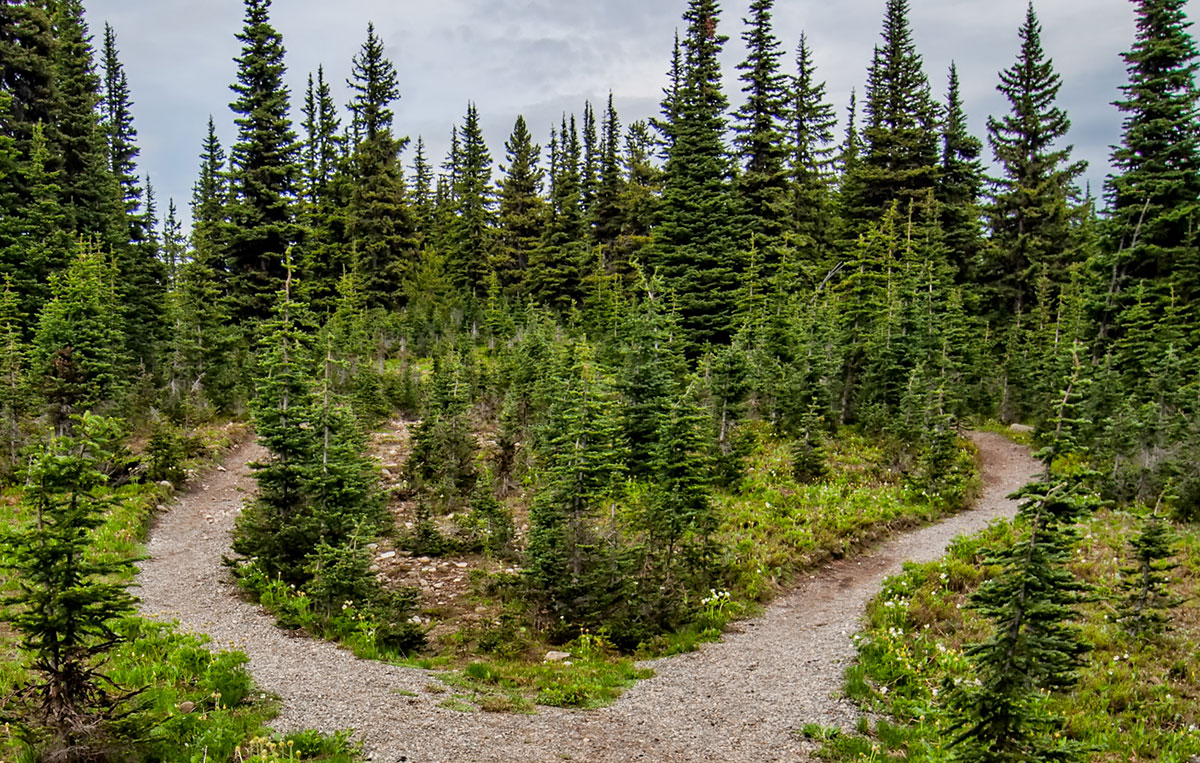
\includegraphics[height=1.05\textheight,keepaspectratio]{nontex/illustrations/forkInRoad.jpg}};}
\begin{frame}
\frametitle{Detailed Refactoring Recommendations}
\end{frame}
}
\note[itemize]{
    \item
}

%------------------------------------------------

\begin{frame}[fragile]
\definecolor{arsenic}{rgb}{0.23, 0.27, 0.29}
\definecolor{asparagus}{rgb}{0.53, 0.66, 0.42}
 \setbeamercolor{block title}{fg=arsenic!10!black,bg=asparagus}
  \setbeamercolor{block body}{parent=normal text,use=block title,
                  bg=block title.bg!25!bg}
\frametitle{LIT Group}
\begin{block}{$\overrightarrow{T4 T1}$ by understandability (E1) and community.}
Example: \cverb![\072\073]! $\Rightarrow$ \cverb![:;]!
\end{block}

\begin{block}{$\overrightarrow{T4 T2}$ by community, and trends in understandability (E8) }
Example: \cverb![\072\073]! $\Rightarrow$ \cverb![\x3A\x3B]!
\end{block}

\begin{block}{$\overrightarrow{T3 T1}$ by community}
Example: \cverb![^]! $\Rightarrow$ \cverb!\^!
\end{block}

\begin{block}{$\overrightarrow{T2 T1}$ by community}
Example: \cverb![\x3A\x3B]! $\Rightarrow$ \cverb![:;]!
\end{block}
\end{frame}


\note[itemize]{
\item[LIT] - $\overrightarrow{T4 T2}$ important for invisibles
}

%------------------------------------------------

\begin{frame}[fragile]
\definecolor{cadetgrey}{rgb}{0.57, 0.64, 0.69}
\definecolor{arsenic}{rgb}{0.23, 0.27, 0.29}
 \setbeamercolor{block title}{fg=arsenic!10!black,bg=cadetgrey}
  \setbeamercolor{block body}{parent=normal text,use=block title,
                  bg=block title.bg!25!bg}
\frametitle{CCC Group}

\begin{block}{$\overrightarrow{C2 C1}$ by community, and trends in understandability (E7).}
Example: \cverb![abcdef]! $\Rightarrow$ \cverb![a-f]!
\end{block}

\begin{block}{$\overrightarrow{C4 C1}$, $\overrightarrow{C5 C1}$ by community.}
Example: \cverb![\w]! $\Rightarrow$ \cverb![0-9a-zA-Z_]!
\\*Example: \cverb!(0|1|2|3|4|5)! $\Rightarrow$ \cverb![0-5]!
\end{block}

\begin{columns}
\column{.5\textwidth}
\begin{block}{$\overrightarrow{C4 C2}$ for community standards.}
Example: \begin{footnotesize}\cverb![\s]! $\Rightarrow$ \cverb![\t\n\r\c\v ]!\end{footnotesize}
\end{block}
\column{.5\textwidth}
\begin{block}{$\overrightarrow{C2 C4}$ for understandability (E4).}
Example: \begin{footnotesize}\cverb![\t\n\r\c\v ]! $\Rightarrow$ \cverb![\s]!\end{footnotesize}
\end{block}
\end{columns}

\begin{columns}
\column{.5\textwidth}
\begin{block}{$\overrightarrow{C5 C2}$ for community standards.}
Example: \cverb!(a|e|i|o|u)! $\Rightarrow$ \cverb![aeiou]!
\end{block}
\column{.5\textwidth}
\begin{block}{$\overrightarrow{C2 C5}$ for understandability (E3).}
Example: \cverb![aeiou]! $\Rightarrow$ \cverb!(a|e|i|o|u)!
\end{block}
\end{columns}

\end{frame}

\note[itemize]{
\item[CCC] - $\overrightarrow{C2 C1}$ only sequences in C2 were tested
\item[C2] - all edges go out of C2! for underst.
\item[C3] - maybe only C4 is possible, for NCCC with NDEC or similar
}

%------------------------------------------------

\begin{frame}[fragile]
\definecolor{copperrose}{rgb}{0.6, 0.4, 0.4}
\definecolor{coolblack}{rgb}{0.0, 0.18, 0.39}
 \setbeamercolor{block title}{fg=coolblack!10!black,bg=copperrose}
  \setbeamercolor{block body}{parent=normal text,use=block title,
                  bg=block title.bg!25!bg}
\frametitle{DBB Group}

\begin{columns}
\column{.5\textwidth}
\begin{block}{$\overrightarrow{D2 D3}$ for understandability (E2).}
Example: \cverb!(ab)?c! $\Rightarrow$ \cverb!abc|c!
\end{block}
\column{.5\textwidth}
\begin{block}{$\overrightarrow{D3 D2}$ for community.}
Example: \cverb!abc|c! $\Rightarrow$ \cverb!(ab)?c!
\end{block}
\end{columns}


\begin{columns}
\column{.5\textwidth}
\begin{block}{$\overrightarrow{D2 D1}$ for understandability (E6).}
Example: \cverb!(ab)?c! $\Rightarrow$ \cverb!(ab){0,1}c!
\end{block}
\column{.5\textwidth}
\begin{block}{$\overrightarrow{D1 D2}$ for community.}
Example: \cverb!(ab){0,1}c! $\Rightarrow$ \cverb!(ab)?c!
\end{block}
\end{columns}

\begin{block}{$\overrightarrow{D3 D1}$ for community.}
Example: \cverb!abc|c! $\Rightarrow$ \cverb!(ab){0,1}c!
\end{block}
\end{frame}


\note[itemize]{
\item[DBB] D3 is likely only good for one QST - not tested for multiple

\item[DBB] E6 is just a trend

\item[DBB] D2 keeps winning because QST is wildly more frequent: 1871 vs 346(D1) and 10(D3)
}

%------------------------------------------------

\begin{frame}[fragile]
\definecolor{peach-orange}{rgb}{1.0, 0.8, 0.6}
\definecolor{paynegrey}{rgb}{0.25, 0.25, 0.28}
 \setbeamercolor{block title}{fg=paynegrey!10!black,bg=peach-orange}
  \setbeamercolor{block body}{parent=normal text,use=block title,
                  bg=block title.bg!25!bg}
\frametitle{LWB, SNG Groups}

\begin{block}{$\overrightarrow{L1 L2}$ by community standard.}
Example: \cverb![a\d]{2,}! $\Rightarrow$ \cverb![a\d][a\d][a\d]*!
\end{block}


\begin{block}{$\overrightarrow{L2 L3}$ for understandability (E5).}
Example: \cverb!ZZ*! $\Rightarrow$ \cverb!Z+!
\end{block}
\begin{center}
SNG community standard is complicated by double-letters in S2.
\\*SNG understandability differences were not significant, only S1 -- S2 measured.
\end{center}
\end{frame}


\note[itemize]{
\item[LWB, SNG] S2 needs to be broken into for-chars and otherwise, or else the char repetitions will swamp interesting data, IMHO
\item [L1 -- L2] not measured for understandability
\item [L2] technically, L2 has 0.23\% more community support than L3, by NRegexes, but then L3 is ahead of L2 by NProjects.  It seems that they are in a tie - a very small change in the mined project set could reverse these leads.
\item
}
